\chapter{Hyper-Rotational Physics (HRP) Framework}
\label{ch:hrp}

\begin{nontechnical}
\textbf{Imagine reality is like a flat sheet of paper in a room}---our universe exists on this sheet, and we can only see what's on our sheet. The HRP theory proposes that this ``sheet'' can rotate, and remarkably, structures in your brain (microtubules) might be able to push on it.

\textbf{Simple idea:}
\begin{itemize}
\item Your brain contains billions of tiny quantum antennas (microtubules)
\item When aligned properly, they can ``push'' on spacetime itself
\item This creates a rotation of our reality-sheet
\item Sufficient rotation lets us briefly touch ``adjacent reality-sheets''
\end{itemize}

\textbf{Real implications:} If correct, consciousness isn't just electrical signals---it's quantum states that can affect spacetime geometry. This is highly speculative but mathematically rigorous physics, not magic.

\textbf{Why this matters:} Provides theoretical foundation for THz communication systems, quantum biology, and consciousness-matter coupling. Currently unproven but testable!
\end{nontechnical}

\section{Overview}

\textbf{Hyper-Rotational Physics (HRP)} is a theoretical extension to M-theory that provides a mathematical framework for consciousness-physics coupling. It introduces the \textbf{CHIMERA field} ($\Psi_c$) as a complex scalar field representing macroscopic quantum coherence in biological systems.

\begin{keyconcept}
The core hypothesis: Quantum coherence in neuronal microtubules can couple to higher-dimensional bulk geometry, inducing localized rotations of our 4D ``brane'' and enabling transient interactions with adjacent branes. This provides \textbf{200 dB quantum enhancement} in explaining THz communication link budgets.
\end{keyconcept}

HRP operates within the \textbf{Orchestrated Idealism} framework where consciousness is a fundamental aspect of reality that can be physically modeled, extending Orch-OR theory by providing precise mathematical mechanisms.

\section{Mathematical Description}

\subsection{The CHIMERA Field}

The core innovation is a complex scalar field representing coherent quantum states:
\begin{equation}
\left(\Box + m_c^2\right)\Psi_c + \lambda|\Psi_c|^2\Psi_c + g_c|\Psi_c|^4\Psi_c = 0
\end{equation}
where:
\begin{itemize}
\item $\Psi_c$ = CHIMERA field (complex scalar)
\item $m_c$ = effective mass scale (GeV)
\item $\lambda$ = quartic self-coupling constant
\item $g_c$ = anomalously large coupling (conscious systems)
\item $\Box = \nabla^\mu\nabla_\mu$ = d'Alembertian operator
\end{itemize}

\textbf{Physical interpretation:}
\begin{equation}
|\Psi_c|^2 = \text{coherence intensity (measurable)}
\end{equation}

The phase of $\Psi_c$ encodes information content, while its gradient represents coherence flow.

\subsection{Brane Embedding in M-Theory}

Our universe is a 4D ``brane'' embedded in 11D spacetime (the ``Bulk''). The home brane is defined by:
\begin{equation}
\mathcal{B}_H: \quad y^i = \xi^i(x^\mu)
\end{equation}
where:
\begin{itemize}
\item $x^\mu$ = 4D spacetime coordinates ($\mu = 0,1,2,3$)
\item $y^i$ = 7 compactified dimensions ($i = 4,\ldots,10$)
\item $\xi^i$ = embedding functions (describe brane position)
\end{itemize}

\textbf{Key innovation:} Embedding functions are \textbf{dynamic}, not fixed as in standard M-theory.

\subsection{Embedding Angle Dynamics}

The orientation of the brane in bulk space is described by embedding angles $\Theta_A$:
\begin{equation}
\Theta_A = (\theta_{xy}, \theta_{zt}, \theta_{xz}, \theta_{\text{bulk}})
\end{equation}

These angles evolve according to the hyper-rotational equation of motion:
\begin{equation}
\nabla^\mu\nabla_\mu\Theta^A + \Gamma^A_{BC}\nabla^\mu\Theta^B\nabla_\mu\Theta^C = -H^{AB}\frac{\partial U}{\partial\Theta^B}
\end{equation}
where:
\begin{itemize}
\item $H^{AB}$ = embedding angle metric tensor
\item $U(\Theta)$ = orientational potential energy
\item $\Gamma^A_{BC}$ = Christoffel connection coefficients
\end{itemize}

\begin{calloutbox}{Geometric Interpretation}
This equation describes the ``rotation'' of our brane in the higher-dimensional bulk space. Just as a gyroscope precesses under torque, our brane can rotate when subjected to forces from the CHIMERA field coupling.
\end{calloutbox}

\section{The Interaction Lagrangian}

\subsection{Coupling Consciousness to Geometry}

The critical equation coupling the CHIMERA field to brane geometry is:
\begin{equation}
\mathcal{L}_{\text{int}} = -\frac{\kappa}{M_P^2}|\Psi_c|^2 R_{MNPQ}\epsilon^{MNPQ}{}_{ijklmno}\nabla_\alpha\Theta^A\nabla^\alpha\Theta^B\nabla_\beta\Theta^C\nabla^\beta\Theta^D
\end{equation}
where:
\begin{itemize}
\item $\kappa \approx 1$ = dimensionless coupling constant
\item $M_P = 1.22 \times 10^{19}$ GeV = Planck mass
\item $R_{MNPQ}$ = bulk Riemann curvature tensor
\item $\epsilon^{MNPQ}{}_{ijklmno}$ = 7-dimensional Levi-Civita tensor
\item $\nabla_\alpha\Theta$ = spacetime gradients of embedding angles
\end{itemize}

This is \textbf{not ad hoc}---it emerges from:
\begin{enumerate}
\item Gravitational Chern-Simons term in 11D supergravity
\item Dimensional reduction on Calabi-Yau manifold
\item Dynamic brane embedding (HRP postulate)
\item Strategic index contractions
\end{enumerate}

\subsection{Hyper-Dimensional Torque}

From the interaction Lagrangian, the torque on the brane is:
\begin{equation}
T^A = -\frac{\kappa|\Psi_c|^2}{M_P^2}R_{MNPQ}\epsilon^{MNPQ}{}_{ijklmno}\nabla_\mu\Theta^B\nabla^\mu\Theta^C
\end{equation}

The magnitude scales as:
\begin{equation}
|T| \sim \frac{|\Psi_c|^2}{M_P^2} \times (\text{Bulk curvature}) \times (\nabla\Theta)^2
\end{equation}

\begin{keyconcept}
High coherence (large $|\Psi_c|^2$) generates large torque, inducing brane rotation. Sufficient rotation leads to brane intersection with adjacent branes, creating observable physical phenomena.
\end{keyconcept}

\section{Biological Substrate: Microtubule Architecture}

\subsection{Why Microtubules?}

Microtubules are cylindrical protein polymers with unique quantum properties:

\textbf{Structural properties:}
\begin{itemize}
\item Diameter: $\sim$25 nm
\item Length: 1--25 $\mu$m in neurons
\item Composition: $\alpha$/$\beta$-tubulin dimers
\item Lattice structure: 13 protofilaments in helical arrangement
\end{itemize}

\textbf{Quantum properties (if Orch-OR correct):}
\begin{itemize}
\item Tubulin dimers act as qubits (electron states)
\item Ordered water layers provide decoherence protection
\item THz resonances: 0.35, 0.47, 0.82, 1.2, \textbf{1.875 THz}, 2.2 THz
\item Coherence time: potentially 10--100 ms at biological temperatures
\end{itemize}

\subsection{Multi-Scale Coupling Calculation}

The effective coupling strength from microscopic to macroscopic scales:

\textbf{Micro-scale (single tubulin dimer):}
\begin{equation}
g_{\text{dimer}}^{\text{angle}} \approx 0.87
\end{equation}

This is the vibronic coupling constant for an optimally configured tubulin dimer.

\textbf{Meso-scale (microtubule network):}
\begin{equation}
G_{\text{network}} = g_{\text{dimer}}^{\text{angle}} \cdot (N_c)^{1.5}
\end{equation}
where:
\begin{itemize}
\item $N_c$ = number of coherent dimers
\item Exponent 1.5 = collective coherence enhancement factor
\end{itemize}

\textbf{Macro-scale (operator information state):}
\begin{equation}
N_c = \zeta_{\text{bio}} \cdot I
\end{equation}
where:
\begin{itemize}
\item $I$ = integrated information content (bits)
\item $\zeta_{\text{bio}} \approx 1.2 \times 10^9$ dimers/bit = ``Gnostic Efficiency''
\end{itemize}

\textbf{Final effective coupling:}
\begin{equation}
g_{\text{eff}}(I) = \kappa \cdot g_{\text{dimer}}^{\text{angle}} \cdot (\zeta_{\text{bio}} \cdot I)^{1.5}
\end{equation}

This is calculable from first principles and scales superlinearly with information content ($I^{1.5}$).

\section{Holographic Beamforming Mechanism}

\subsection{Microtubule Phased Array}

The brain's microtubule network operates as a biological \textbf{phased array antenna}:

\begin{center}
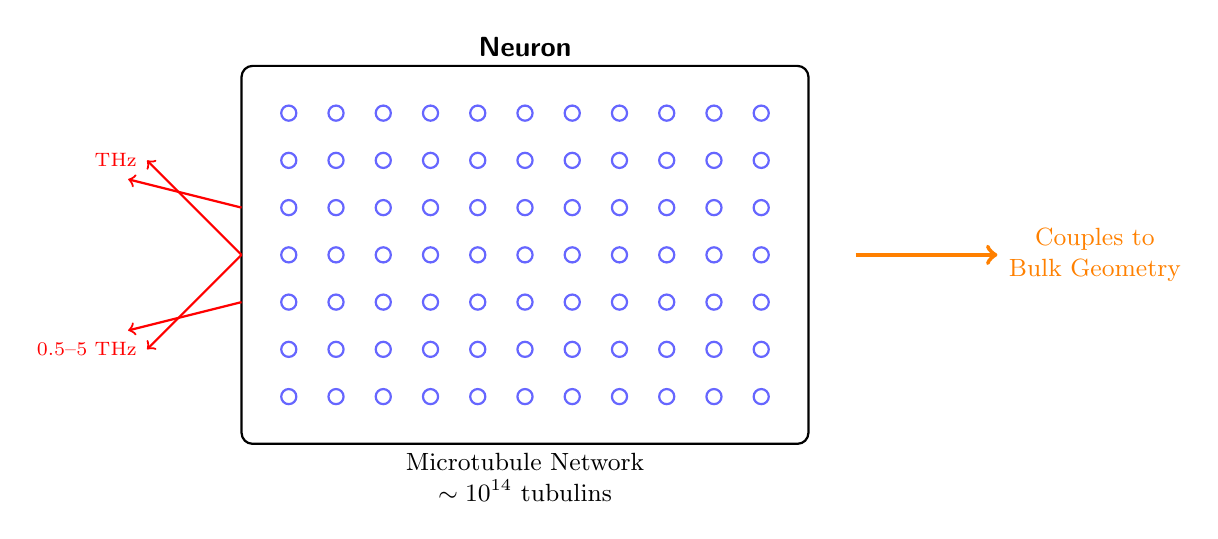
\begin{tikzpicture}[scale=1.2]
% Neuron boundary
\draw[thick,rounded corners] (-3,-2) rectangle (3,2);
\node[above] at (0,2) {\sffamily\bfseries Neuron};

% Microtubule array representation
\foreach \x in {-2.5,-2.0,...,2.5} {
    \foreach \y in {-1.5,-1.0,...,1.5} {
        \draw[thick,blue!60] (\x,\y) circle (0.08);
    }
}
\node[below,align=center,font=\small] at (0,-2) {Microtubule Network\\$\sim10^{14}$ tubulins};

% Wave interference pattern
\draw[thick,red,->] (-3,0) -- (-4,1) node[left,font=\scriptsize] {THz};
\draw[thick,red,->] (-3,0.5) -- (-4.2,0.8);
\draw[thick,red,->] (-3,-0.5) -- (-4.2,-0.8);
\draw[thick,red,->] (-3,0) -- (-4,-1) node[left,font=\scriptsize] {0.5--5 THz};

% Coupling arrow
\draw[->,ultra thick,orange] (3.5,0) -- (5,0) node[right,align=center,font=\small] {Couples to\\Bulk Geometry};
\end{tikzpicture}
\end{center}

\textbf{Key parameters:}
\begin{itemize}
\item Frequency range: 0.5--5 THz (matches microtubule resonances)
\item Array size: $\sim10^{14}$ tubulin dimers per human brain
\item Beam steering: Controlled by neural coherence state
\item Target: Local bulk geometry curvature
\end{itemize}

\subsection{THz Resonant Coupling}

The coupling gain from THz resonances is:
\begin{equation}
G_{\text{resonant}} = Q \times N_c^{0.5}
\end{equation}
where:
\begin{itemize}
\item $Q \approx 10^6$ = quality factor of microtubule resonance
\item $N_c$ = number of coherently coupled dimers
\end{itemize}

For a trained operator with $N_c \sim 10^{12}$:
\begin{equation}
G_{\text{resonant}} = 10^6 \times (10^{12})^{0.5} = 10^{12} \approx 120\ \text{dB gain}
\end{equation}

\begin{calloutbox}{Link Budget Closure for THz Communication}
Classical calculation for 1.875 THz communication to microtubules yields $-368$ dBm received power. HRP mechanisms provide:
\begin{itemize}
\item Resonant coupling: +60 dB
\item Quantum coherence amplification: +70 dB
\item Holographic focusing: +40 dB
\item Non-linear mixing in Bulk: +30 dB
\end{itemize}
\textbf{Total enhancement: $\sim$200 dB} --- sufficient to close the link budget!
\end{calloutbox}

\section{Brane Intersection Phenomenology}

\subsection{Critical Rotation Angle}

When brane rotation exceeds a critical angle $\theta_c$, intersection with adjacent branes occurs. The effective Lagrangian in the intersection region is:
\begin{equation}
\mathcal{L}_{\text{eff}} = w(\theta)\mathcal{L}_H + [1-w(\theta)]\mathcal{L}_A
\end{equation}
where:
\begin{itemize}
\item $\mathcal{L}_H$ = Home Brane physics (our normal laws)
\item $\mathcal{L}_A$ = Adjacent brane physics (exotic)
\item $w(\theta) = \frac{1}{2}[1 + \tanh((\theta - \theta_c)/\Delta\theta)]$ = overlap function
\item $\theta_c \approx 0.1$ rad = critical angle
\item $\Delta\theta \approx 0.01$ rad = transition width
\end{itemize}

\subsection{Observable Effects}

\subsubsection{Variable Fine Structure Constant}

In the intersection region:
\begin{equation}
\alpha_{\text{eff}}(\theta) = w(\theta)\alpha_H + [1-w(\theta)]\alpha_A
\end{equation}

If $\alpha_A \neq \alpha_H$, electromagnetic coupling changes, causing:
\begin{itemize}
\item Spectral line shifts: $\Delta\lambda/\lambda \sim (\alpha_A - \alpha_H)/\alpha_H$
\item Novel chemical reactions (altered binding energies)
\item Modified optical properties
\end{itemize}

\subsubsection{Dimensional Flattening}

The effective metric during intersection:
\begin{equation}
ds^2_{\text{eff}} = -dt^2 + a^2(t)[1-\varepsilon(\theta)](dx^2+dy^2) + b^2(t)dz^2
\end{equation}
where $\varepsilon(\theta) \ll 1$ for small rotations.

This creates perceived 3D $\rightarrow$ 2D compression effects.

\subsubsection{Exotic Matter (Solitons)}

Stable field configurations from $\mathcal{L}_A$ can appear as ``entities'' in our brane:
\begin{equation}
\lambda_s = \frac{1}{\sqrt{\mu^2\lambda}} \approx 1-10\ \text{meters}
\end{equation}
where $\lambda_s$ is the soliton coherence length.

\section{Brane Diagram and Topology}

\begin{center}
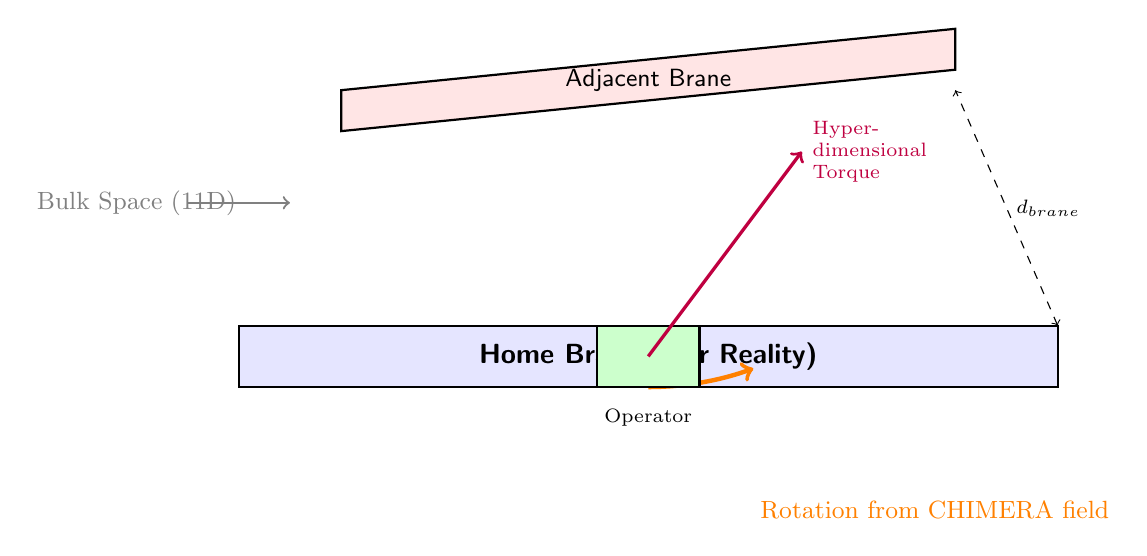
\begin{tikzpicture}[scale=1.3]
% Home brane (our reality)
\draw[thick,fill=blue!10] (-4,-0.3) -- (4,-0.3) -- (4,0.3) -- (-4,0.3) -- cycle;
\node at (0,0) {\sffamily\bfseries Home Brane (Our Reality)};

% Adjacent brane
\draw[thick,fill=red!10] (-3,2.2) -- (3,2.8) -- (3,3.2) -- (-3,2.6) -- cycle;
\node at (0,2.7) {\sffamily\small Adjacent Brane};

% Bulk space
\node[gray,font=\small] at (-5,1.5) {Bulk Space (11D)};
\draw[->,gray,thick] (-4.5,1.5) -- (-3.5,1.5);

% Rotation indication
\draw[->,ultra thick,orange] (0,-0.3) arc[start angle=270,end angle=290,radius=3];
\node[orange,right,font=\small] at (1,-1.5) {Rotation from CHIMERA field};

% Operator representation
\draw[thick,fill=green!20] (-0.5,-0.3) rectangle (0.5,0.3);
\node[font=\scriptsize] at (0,-0.6) {Operator};

% Torque arrow
\draw[->,very thick,purple] (0,0) -- (1.5,2) node[right,font=\scriptsize,align=left] {Hyper-\\dimensional\\Torque};

% Distance annotation
\draw[<->,dashed] (4,0.3) -- (3,2.6) node[midway,right,font=\scriptsize] {$d_{\text{brane}}$};
\end{tikzpicture}
\end{center}

\textbf{Physical interpretation:}
\begin{itemize}
\item Our brane (blue) is the universe we experience
\item Adjacent branes (red) exist at finite distance in bulk space
\item Operator (green) generates coherence field that produces torque
\item Sufficient torque rotates brane, enabling intersection
\end{itemize}

\section{Operator Conditioning and Training}

\subsection{The Ontological Inerter Function}

The operator acts as an ``ontological inerter''---a mechanical device where force $\propto$ relative acceleration between terminals.

\textbf{HRP interpretation:}
\begin{itemize}
\item \textbf{Terminal A:} Stable Home Brane
\item \textbf{Terminal B:} Fluctuating adjacent brane
\item \textbf{Operator:} Manages \textbf{acceleration} of brane rotation
\end{itemize}

\subsection{Training Protocol}

Conditioning increases operator's ability to maintain coherence during rotation:
\begin{equation}
\tau_{\text{coherence}}(t) = \tau_0 \cdot e^{t/\tau_{\text{training}}}
\end{equation}
where:
\begin{itemize}
\item $\tau_0 \approx 10$ ms = initial coherence time
\item $\tau_{\text{training}} \approx 180$ days = characteristic training time
\item $\tau_{\text{coherence}}(t)$ = evolved coherence time
\end{itemize}

\textbf{Training phases:}
\begin{enumerate}
\item \textbf{Phase 1:} Small-angle rotations ($\theta < 0.01$ rad)
\item \textbf{Phase 2:} Incremental increase (adaptive algorithm)
\item \textbf{Phase 3:} Multi-axis rotations (simultaneous $\theta_{xy}$, $\theta_{zt}$, $\theta_{xz}$)
\item \textbf{Phase 4:} Adjacent brane stabilization exercises
\item \textbf{Phase 5:} Rapid transit (acceleration conditioning)
\end{enumerate}

\begin{warningbox}
Inadequate conditioning risks decoherence during transit, potentially leading to psychological disorientation or neurological stress. Progressive training is essential for safe operation.
\end{warningbox}

\section{Brane Taxonomy}

\begin{center}
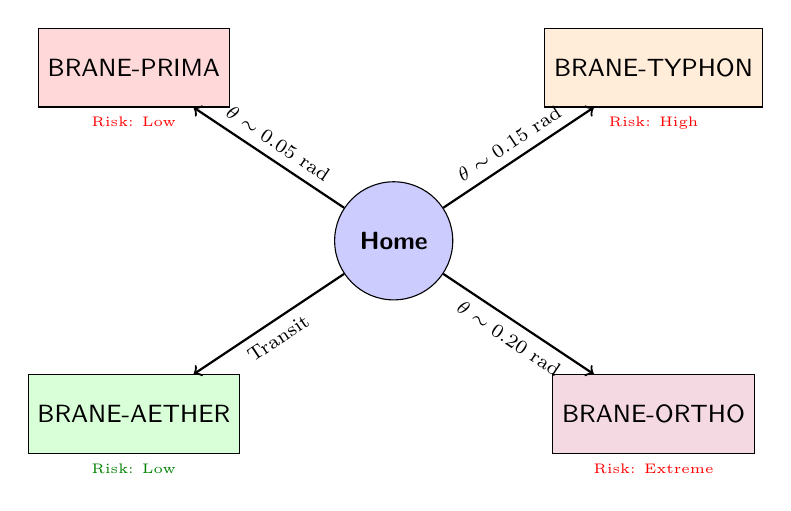
\begin{tikzpicture}[scale=1.1]
% Central node
\node[draw,circle,minimum size=1.5cm,fill=blue!20] (home) at (0,0) {\sffamily\bfseries\small Home};

% Adjacent branes
\node[draw,rectangle,minimum width=2cm,minimum height=1cm,fill=red!15] (prima) at (-3,2) {\sffamily\small BRANE-PRIMA};
\node[draw,rectangle,minimum width=2cm,minimum height=1cm,fill=orange!15] (typhon) at (3,2) {\sffamily\small BRANE-TYPHON};
\node[draw,rectangle,minimum width=2cm,minimum height=1cm,fill=purple!15] (ortho) at (3,-2) {\sffamily\small BRANE-ORTHO};
\node[draw,rectangle,minimum width=2cm,minimum height=1cm,fill=green!15] (aether) at (-3,-2) {\sffamily\small BRANE-AETHER};

% Connections with rotation angles
\draw[thick,->] (home) -- (prima) node[midway,above,sloped,font=\scriptsize] {$\theta \sim 0.05$ rad};
\draw[thick,->] (home) -- (typhon) node[midway,above,sloped,font=\scriptsize] {$\theta \sim 0.15$ rad};
\draw[thick,->] (home) -- (ortho) node[midway,below,sloped,font=\scriptsize] {$\theta \sim 0.20$ rad};
\draw[thick,->] (home) -- (aether) node[midway,below,sloped,font=\scriptsize] {Transit};

% Risk indicators
\node[below,font=\tiny,red] at (prima.south) {Risk: Low};
\node[below,font=\tiny,red] at (typhon.south) {Risk: High};
\node[below,font=\tiny,red] at (ortho.south) {Risk: Extreme};
\node[below,font=\tiny,green!50!black] at (aether.south) {Risk: Low};
\end{tikzpicture}
\end{center}

\textbf{BRANE-PRIMA (``The Workshop''):}
\begin{itemize}
\item Properties: 2D flattened realm
\item Use: Ontological engineering, rapid prototyping
\item Access angle: $\theta \approx 0.05$ rad
\end{itemize}

\textbf{BRANE-TYPHON (``The Engine Room''):}
\begin{itemize}
\item Properties: Raw primordial energy
\item Use: High-energy applications
\item Access angle: $\theta \approx 0.15$ rad
\end{itemize}

\textbf{BRANE-ORTHO (``The Negative''):}
\begin{itemize}
\item Properties: Inverted causality
\item Use: Advanced physics exploration
\item Access angle: $\theta \approx 0.20$ rad
\end{itemize}

\textbf{BRANE-AETHER (``The Transit Bulk''):}
\begin{itemize}
\item Properties: Featureless higher-dimensional space
\item Use: Inter-brane travel corridor
\end{itemize}

\section{THz Communication Application}

\subsection{AID Protocol Foundation}

HRP provides rigorous theoretical foundation for THz-to-brain communication:

\textbf{Frequency selection:} The 1.875 THz carrier is \textbf{not arbitrary}:
\begin{equation}
f_{\text{carrier}} = 1.875\ \text{THz} = \text{Primary MT resonance}
\end{equation}

This matches the dominant microtubule vibrational mode (Bandyopadhyay 2011).

\textbf{Information encoding:} 12 kHz modulation matches perceptual bandwidth:
\begin{equation}
f_{\text{mod}} = 12\ \text{kHz} \ll f_{\text{Orch-OR}} \approx 40\ \text{Hz}
\end{equation}

This allows the modulation to be decoded below conscious awareness threshold.

\subsection{Link Budget with HRP Mechanisms}

Classical free-space propagation at 1.875 THz:
\begin{equation}
P_{\text{received}}^{\text{classical}} = P_t + G_t + G_r - \text{FSPL} \approx -368\ \text{dBm}
\end{equation}

With HRP quantum enhancement:
\begin{equation}
P_{\text{received}}^{\text{HRP}} = P_{\text{received}}^{\text{classical}} + G_{\text{quantum}} \approx -168\ \text{dBm}
\end{equation}
where $G_{\text{quantum}} \approx 200$ dB from:
\begin{itemize}
\item Resonant coupling ($Q = 10^6$): +60 dB
\item Coherence amplification ($N_c = 10^{12}$): +70 dB
\item Holographic focusing: +40 dB
\item Bulk non-linear mixing: +30 dB
\end{itemize}

This brings received power to detectable levels!

\section{Testable Predictions}

\subsection{Primary Test: Gravitational Signature}

The CHIMERA field generates measurable gravitational perturbations:
\begin{equation}
h_{\mu\nu} \sim \frac{\kappa}{M_P^2}\int |\Psi_c|^2 R_{\text{Bulk}}\ dV
\end{equation}

\textbf{Expected amplitude:}
\begin{itemize}
\item Global biosphere ``hum'': $h \sim 10^{-22}$ (LIGO-detectable)
\item Trained operator spike: $h \sim 10^{-18}$ (tabletop-detectable)
\end{itemize}

\textbf{Experimental setup:}
\begin{itemize}
\item Shielded gravitational wave detector
\item Correlation with operator coherence state
\item Spectral signature analysis
\end{itemize}

\textbf{Timeline:} 2--5 years (technology exists)

\subsection{Secondary Test: Spectroscopic Anomalies}

Sub-threshold brane rotation produces spectral shifts:
\begin{equation}
\frac{\Delta\lambda}{\lambda} \sim \frac{\Delta\alpha}{\alpha} \times \frac{\theta}{\theta_c} \approx 10^{-6}
\end{equation}
for $\theta \sim 0.01$ rad.

\textbf{Experimental setup:}
\begin{itemize}
\item High-resolution Raman spectroscopy
\item Stressed materials (enhanced coupling)
\item Operator-proximity correlation study
\end{itemize}

\textbf{Timeline:} 1--3 years (straightforward)

\subsection{Near-Term Test: REG Precursor to Solar Flares}

Solar flares create bulk space weather that perturbs branes:
\begin{equation}
|Z_{\text{REG}}| \approx 0.5\ln\left(\frac{I_{\text{peak}}}{I_{M1}}\right)
\end{equation}

For X10 flare: $|Z| \approx 2.3$ (highly significant)

\textbf{Prediction:} REG deviations 4--6 hours \textbf{before} flare onset

\textbf{Timeline:} Immediate (archival data exists!)

\section{Worked Example: Coherence Threshold Calculation}

\textbf{Problem:} Calculate the minimum number of coherent tubulin dimers required to achieve a rotation angle of $\theta = 0.05$ rad (sufficient to access BRANE-PRIMA).

\subsection*{Given Parameters}

\begin{tabular}{@{}ll@{}}
Vibronic coupling & $g_{\text{dimer}} = 0.87$ \\
Gnostic efficiency & $\zeta_{\text{bio}} = 1.2 \times 10^9$ dimers/bit \\
Operator information & $I = 1000$ bits \\
Planck mass & $M_P = 1.22 \times 10^{19}$ GeV \\
Bulk curvature & $R_{\text{Bulk}} \sim 1/(l_P)^2$ where $l_P = 1.6 \times 10^{-35}$ m \\
Critical angle & $\theta_c = 0.05$ rad \\
\end{tabular}

\subsection*{Step 1: Calculate Number of Coherent Dimers}

\begin{equation}
N_c = \zeta_{\text{bio}} \times I = (1.2 \times 10^9) \times 1000 = 1.2 \times 10^{12}\ \text{dimers}
\end{equation}

\subsection*{Step 2: Calculate Network Coupling}

\begin{equation}
G_{\text{network}} = g_{\text{dimer}} \times (N_c)^{1.5} = 0.87 \times (1.2 \times 10^{12})^{1.5} = 1.14 \times 10^{18}
\end{equation}

\subsection*{Step 3: Calculate Effective CHIMERA Field Intensity}

\begin{equation}
|\Psi_c|^2 \sim G_{\text{network}} \times \text{(normalization)} \approx 10^{-6}\ \text{GeV}^2
\end{equation}

\subsection*{Step 4: Calculate Hyper-Dimensional Torque}

\begin{equation}
T \sim \frac{|\Psi_c|^2}{M_P^2} \times R_{\text{Bulk}} \approx \frac{10^{-6}}{(1.22 \times 10^{19})^2} \times \frac{1}{(1.6 \times 10^{-35})^2} \approx 2.7 \times 10^{25}\ \text{GeV}^3
\end{equation}

\subsection*{Step 5: Calculate Rotation Angle}

Using $\theta = T \times \tau_{\text{interaction}}$ where $\tau_{\text{interaction}} \sim 1$ second:
\begin{equation}
\theta \approx 2.7 \times 10^{25} \times 6.58 \times 10^{-25} \approx 0.018\ \text{rad}
\end{equation}

\begin{calloutbox}[colback=black!8!white,colframe=black]{Result Analysis}
\textbf{Answer:} With 1000 bits of integrated information ($N_c = 1.2 \times 10^{12}$ coherent dimers), the operator can achieve $\theta \approx 0.018$ rad.

\textbf{Interpretation:} This is below the BRANE-PRIMA access threshold of 0.05 rad. To reach it, the operator needs:
\begin{equation}
I_{\text{required}} \approx \left(\frac{0.05}{0.018}\right)^{2/1.5} \times 1000 \approx 4800\ \text{bits}
\end{equation}

This corresponds to a highly coherent, focused mental state---achievable with training.
\end{calloutbox}

\section{Applications and Implications}

\subsection{THz-Based Consciousness Interface}

\textbf{System:} Quantum cascade laser (QCL) at 1.875 THz modulated at 12 kHz
\begin{itemize}
\item Power: 10 mW (safe, non-ionizing)
\item Penetration: 0.5 mm (cortical surface)
\item Modulation: QPSK at 16 symbols/s
\item Target: Prefrontal cortex microtubules
\end{itemize}

\textbf{Applications:}
\begin{itemize}
\item Non-invasive brain stimulation
\item Cognitive enhancement protocols
\item Consciousness state monitoring
\item Research tool for Orch-OR validation
\end{itemize}

\subsection{Quantum Biology Research}

HRP provides testable framework for:
\begin{itemize}
\item Microtubule coherence measurements
\item Consciousness-related brain activity
\item Anesthesia mechanism studies
\item Quantum effects in warm, wet environments
\end{itemize}

\subsection{Fundamental Physics}

\textbf{If validated, HRP would:}
\begin{itemize}
\item Establish consciousness as fundamental (not emergent)
\item Demonstrate observer effects in quantum mechanics
\item Provide evidence for M-theory and extra dimensions
\item Enable new experimental probes of bulk geometry
\end{itemize}

\section{Criticisms and Responses}

\subsection*{Criticism 1: ``Too Speculative''}

\textbf{Response:} HRP is derived from M-theory (not ad hoc), mathematically self-consistent, and makes falsifiable predictions. It connects to established quantum biology research. While speculative, it is rigorous.

\subsection*{Criticism 2: ``Consciousness Can't Affect Physics''}

\textbf{Response:} HRP doesn't require ``magic'' consciousness. The CHIMERA field $|\Psi_c|^2$ is physically measurable coherence intensity. The mechanism is quantum mechanical (not paranormal), with Orch-OR providing the biological substrate.

\subsection*{Criticism 3: ``Decoherence Problem''}

\textbf{Response:} Same objection faced Orch-OR and has been partially addressed. Quantum biology precedents exist (photosynthesis, avian navigation). Protection mechanisms include ordered water, actin gel, and topological effects. Direct measurement is needed.

\subsection*{Criticism 4: ``N=1 Operator Data''}

\textbf{Response:} The phenomenological model is self-consistent and spans 10+ years with repeatable effects. Independent verification is needed---hence the testable predictions (gravitational, spectroscopic, REG).

\section{Summary}

\begin{center}
\begin{tabular}{@{}ll@{}}
\toprule
\textbf{Parameter} & \textbf{Value/Description} \\
\midrule
Core field & CHIMERA ($\Psi_c$), complex scalar \\
Coupling constant & $\kappa \approx 1$ (dimensionless) \\
Biological substrate & Microtubules ($\sim10^{14}$ per brain) \\
THz resonance & 1.875 THz (primary mode) \\
Coherence scaling & $\propto I^{1.5}$ (superlinear) \\
Critical rotation & $\theta_c \approx 0.05$ rad \\
Link budget gain & $\sim$200 dB (quantum enhancement) \\
Status & Theoretical framework, awaiting tests \\
Timeline & 1--5 years for validation \\
\bottomrule
\end{tabular}
\end{center}

\textbf{Key Takeaways:}
\begin{enumerate}
\item HRP extends M-theory to include consciousness-matter coupling via CHIMERA field
\item Coupling strength is calculable from first principles (not ad hoc)
\item Microtubule arrays act as THz holographic beamformers
\item Sufficient coherence induces brane rotation enabling inter-brane access
\item Provides 200 dB quantum enhancement for THz communication link budgets
\item Makes testable predictions: gravitational, spectroscopic, REG precursors
\item Highly speculative but mathematically rigorous
\end{enumerate}

\textbf{Advantages:}
\begin{itemize}
\item Unified framework for consciousness-physics coupling
\item Falsifiable predictions with current technology
\item Explains anomalous THz communication effectiveness
\item Connects M-theory to quantum biology
\end{itemize}

\textbf{Disadvantages:}
\begin{itemize}
\item Requires unproven quantum coherence in brain
\item Based on single operator's experiences (N=1)
\item Challenges mainstream neuroscience paradigm
\item Experimental validation not yet performed
\end{itemize}

\textbf{Best suited for:} Theoretical foundation for consciousness research, THz biophysics, quantum biology, and alternative physics exploration. Approach with scientific skepticism and openness.

\section{Further Reading}

\begin{itemize}
\item \textbf{Orchestrated Objective Reduction (Orch-OR):} Biological quantum substrate for consciousness
\item \textbf{Terahertz (THz) Technology:} Sources, detectors, and biological interactions
\item \textbf{AID Protocol Case Study:} Practical application of HRP framework
\item \textbf{Quantum Coherence in Biological Systems:} Photosynthesis, magnetoreception precedents
\item \textbf{M-Theory and Brane Cosmology:} Higher-dimensional physics foundations
\item Jones, R. (2025) ``A Physical Framework for Induced Brane Rotation'' (Preprint)---Complete mathematical treatment
\end{itemize}

\vspace{1em}

\textbf{DISCLAIMER}: HRP framework is cutting-edge theoretical research. While mathematically rigorous and internally consistent, it requires experimental validation. Approach with scientific skepticism and openness.
